
\section{Data modelling II}
%------------------------------------------------------------------------------
\begin{frame}[standout]
    Re: \\ \alert{Data modelling} \\
    (but more technical now)
\end{frame}
%------------------------------------------------------------------------------
\begin{frame}{Data modelling}
\subsection{Definitions and theory}
\metroset{block=fill}
\begin{block}{Representation of originals (attributes)}
\begin{itemize}
    \item image (photo, drawing, diagram etc.)
    \item text 
    \item lists, tables
    \item audio 
    \item objects (experimental setup, sculpture, 3D print, etc.)
\end{itemize}
\end{block}


\begin{block}{What is data modelling?}
\begin{itemize}
    \item \textbf{data:} What does `data' mean?
    \item \textbf{modelling:} What does `data modelling' mean?
\end{itemize}
\end{block}

\end{frame}

%------------------------------------------------------------------------------
\begin{frame}[allowframebreaks]{Data}
\metroset{block=fill}
\begin{block}{Definitions of `data'}
    \begin{enumerate}\footnotesize
        \item Plural of Latin \emph{datum} ('given'): data often isn't exactly a given but a construct: data is created rather than given
        \item  \lbrack{}number\rbrack{}values, findings features, statements, details (collected/created through observation, measurement, statistical polls, phenomenotechnical devices)
        \item (IT) digital numbers, information 
        \item (maths) values given to solve an equation 
    \end{enumerate}
\end{block}

\begin{block}{ISO definitions = standard}\scriptsize
\begin{itemize}
    \item ISO/IEC 2382:2015(en): Information technology -- Vocabulary 2121272 data
    \item \textbf{Reinterpretable representation of information in a formalized manner suitable for communication, interpretation, or processing}
    \item Note 1 to entry: Data can be processed by humans or by automatic means (\href{https://www.iso.org/obp/ui/\#iso:std:iso-iec:2382:ed-1:v1:en}{source})
\end{itemize}
\end{block}

\framebreak
    \begin{block}{Data models}
    \begin{quote}
        Data models are models in the sense of Stachowiak's three main features of a mode but they have one more property: Models generally aren't necessarily computer-processable. To achieve this, they need to be given in an unambiguous, explicit way. Only then can they be machine-processed and only then are they formal models. 
        ~\parencite[100][translated from German]{JannidisIntroDatamod}
        %Datenmodelle sind Modelle in diesem Sinne \lbrack{}3 Hauptmerkmale nach Stachowiak\rbrack{}, aber es kommt eine weitere Eigenschaft hinzu. Modelle im Allgemeinen sind nicht automatisch von Computern prozessierbar. Um das zu erreichen, müssen sie in einer eindeutigen und expliziten Form vorliegen. Erst so können sie vom Computer verarbeitet werden und erst dann sind es formale Modelle. ~\parencite[100][translated from German]{JannidisIntroDatamod}
    \end{quote}
    \end{block}
\end{frame}

%------------------------------------------------------------------------------
\begin{frame}[allowframebreaks]{Digital data representation}
$\to$ i.e. \alert{computer processable}
\metroset{block=fill}
\begin{block}{Digital representation}
    \begin{itemize}
        \item \textbf{images} 
        \begin{itemize}
            \item raster graphics (\texttt{.png}, \texttt{.jpeg}) 
            \item vector graphics (\texttt{.svg})
        \end{itemize}
        \item \textbf{Text}
        \begin{itemize}
            \item plain text (\texttt{.txt})
            \item formatted text (\texttt{.docx})
        \end{itemize}
        \item \textbf{Lists, tables} (\texttt{.csv}, \texttt{.xlsx})
        \item \textbf{Audio} (\texttt{.wav}, \texttt{.midi})
        \item \textbf{Objects:} (Simulation of) three dimensionality and physical attributes
    \end{itemize}
\end{block}
\framebreak 

\begin{block}{For advanced froms of digital representation $\to$ see other ZIM classes}
\begin{itemize}
    \item \textbf{markup languages/OHCO} (\texttt{.xml}, etc.)
    \item \textbf{data objects} (\texttt{.json}, etc.) 
    \item \textbf{graph databases} (\texttt{.rdf}, etc.)
    \item \textbf{relational databases} $\to$ SQL (will follow soon\dots)
\end{itemize}
\end{block}
\end{frame}

%------------------------------------------------------------------------------
\begin{frame}{Fotis Jannidis' phases of data modelling}
\metroset{block=fill}
    \begin{alertblock}{1) conceptual data model}\footnotesize
        \begin{enumerate}
            \item identify relevant entities and their attributes and relations	$\to$ relevant concerning their intended use
            \item visualize entities, attributes and relations in a suitable format $\to$ lists, tables, diagrams (e.g. Entity Relationship Diagramm)
        \end{enumerate}
    \end{alertblock}
    \begin{alertblock}{2) logical data model}
        Map the conceptual model onto the structure of a specific technology, e.g. database schema or XML schema 
    \end{alertblock}
    \begin{alertblock}{3) physical data model}
        Implementation and physical representation of the data model in the memory of a computer as a specific data structure 
    \end{alertblock}
\end{frame}
%------------------------------------------------------------------------------
\begin{frame}{Jannidis, example diagram}
    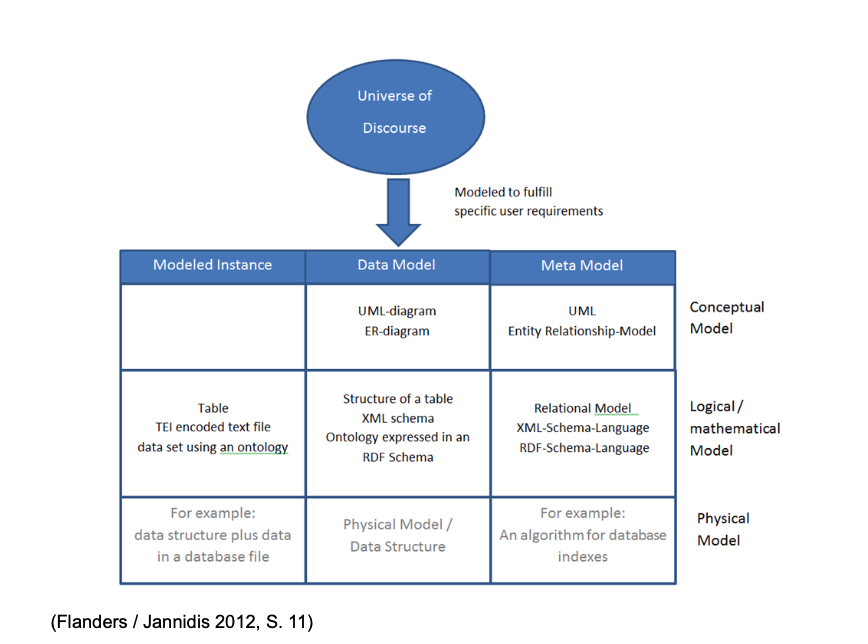
\includegraphics[width=\textwidth]{img/jannidis-modell.png}
\end{frame}

%------------------------------------------------------------------------------
\begin{frame}[fragile]{Example: csv data format (=comma separated values)}
\subsection{csv data format (=comma separated values \texttt{.csv})}
    \begin{enumerate}
        \item simple exchange format for sheet calculation software 
        \item cells (attributes) are separated by a separator character (such as comma, semicolon, tab, etc.)
        \item entries (datasets) separated by newline/line break
        \item fields can be named using headers (optional)
    \end{enumerate}
    \textbf{Source:} \protect\url{ietf.org}, \protect\url{https://tools.ietf.org/html/rfc4180}
    
    \metroset{block=fill}
    \begin{block}{csv example: birth place}\scriptsize
    \begin{verbatim}
    "Name","Address","Description","Longitude","Latitude"
    "forname surname","example street 1, postcode","birth place","7.018242","50.678667"
    \end{verbatim}
    \end{block}
\end{frame}



%------------------------------------------------------------------------------
\section{Entity Relationship Model (ERM)}
%------------------------------------------------------------------------------

%------------------------------------------------------------------------------
\begin{frame}{Entity Relationship Model (by Peter Chen)}
\metroset{block=fill}
\begin{block}{\cite[9]{chen1976}}
    \begin{quote}
        The entity-relationship model can be used as a basis for unification of different views of data: the network model, the relational model, and the entity set model.~
    \end{quote}
\end{block}
\begin{block}{\cite[10]{chen1976}}
    \begin{quote}
        \lbrack{}His article\rbrack{} analyzes the network model, the relational model, and the entity set model, and describes how they may be derived from the entity relationship model.~
    \end{quote}
\end{block}
\begin{block}{\cite[19]{chen1976}}
    \begin{quote}
        \lbrack{}The article presents:\rbrack{} a diagrammatic technique for exhibiting entities and relationships: the entity-relationship diagram.~%\parencite[19]{chen1976}
    \end{quote}
\end{block}
$\to$ \alert{Conceptual model}

\end{frame}

%------------------------------------------------------------------------------
\begin{frame}{ER terminology~\parencite[9--12]{chen1976}}
    % ----------------------------------------------
  \begin{columns}[T,onlytextwidth]
  \metroset{block=fill}
    \column{0.55\textwidth}\footnotesize
      \begin{block}{Entity (Entität)}
       An entity is a „thing“ which can be distinctly identified. A specific person, company, or event is an example of en entity.
      \end{block}

      \begin{alertblock}{Relationship (Beziehung)}
        A relationship is an association among entites. For instance, „father-son“ is a relationship between two „person“ enitities.
      \end{alertblock}

      \begin{exampleblock}{Entity Set (Entitätsmenge)}
        All entities of the same entity set have the same properties.
        %Alle Entitäten derselben Entitätsmenge haben dieselben Eigenschaften (properties). 
        
        „Entities are classified into different entity sets such as EMPLOYEE, PROJECT, and DEPARTMENT.“
      \end{exampleblock}

    % ----------------------------------------------

    \column{0.4\textwidth}

      \metroset{block=fill}

      \begin{block}{ER model elements}
      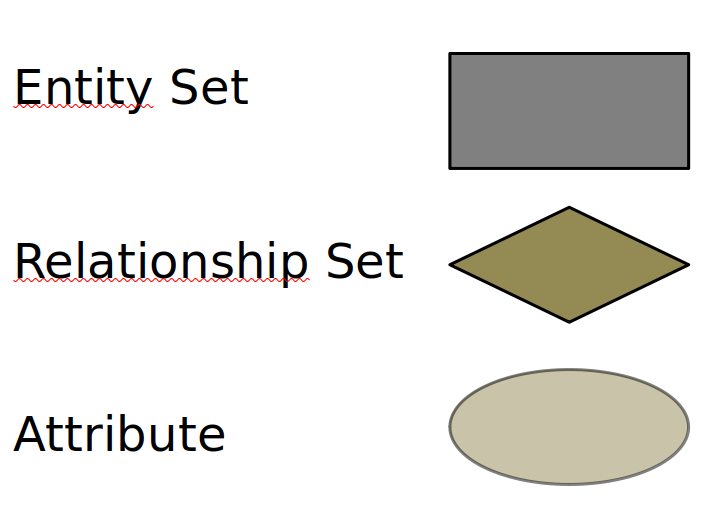
\includegraphics[width=0.9\textwidth]{img/er-modell.png}
      \end{block}
      
      \begin{block}{ER elements}
      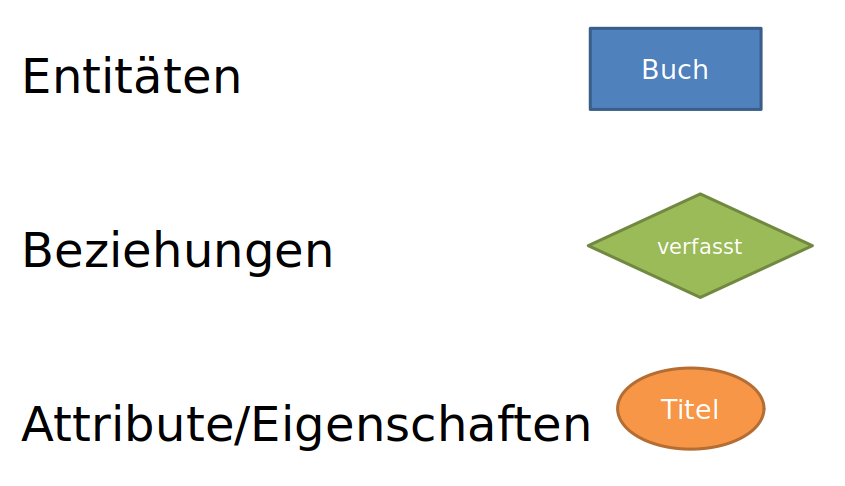
\includegraphics[width=0.9\textwidth]{img/er-bsp2.png}
      \end{block}
  \end{columns}

\end{frame}

%------------------------------------------------------------------------------
\begin{frame}{ER terminology~\parencite[9--12]{chen1976}}
    % ----------------------------------------------
  \begin{columns}[T,onlytextwidth]
  \metroset{block=fill}
    \column{0.48\textwidth}\footnotesize
      \begin{exampleblock}{set of relations (Relationship Set)}
        Same relationships between entities from the same entity sets: can be summarized in a set of relationships.
        %Gleiche Beziehungen zwischen Entitäten, die jeweils aus derselben Entitätsmenge stammen, lassen sich in einer Menge von Beziehungen zusammenfassen. 
      \end{exampleblock}

    % ----------------------------------------------

    \column{0.48\textwidth}

      \metroset{block=fill}
      \begin{block}{Role (Rolle)} \footnotesize
        The role of an entity in a relationship is the function that it performs in the relationship.
      \end{block}
      
      \begin{alertblock}{Properties (Eigenschaften)}\footnotesize
        Using properties, entities and relationships can be described. 
        %Mithilfe von Eigenschaften lassen sich Entitäten (Entities) und Beziehungen (Relationships) beschreiben. 
      \end{alertblock}
  \end{columns}
  \begin{center}
      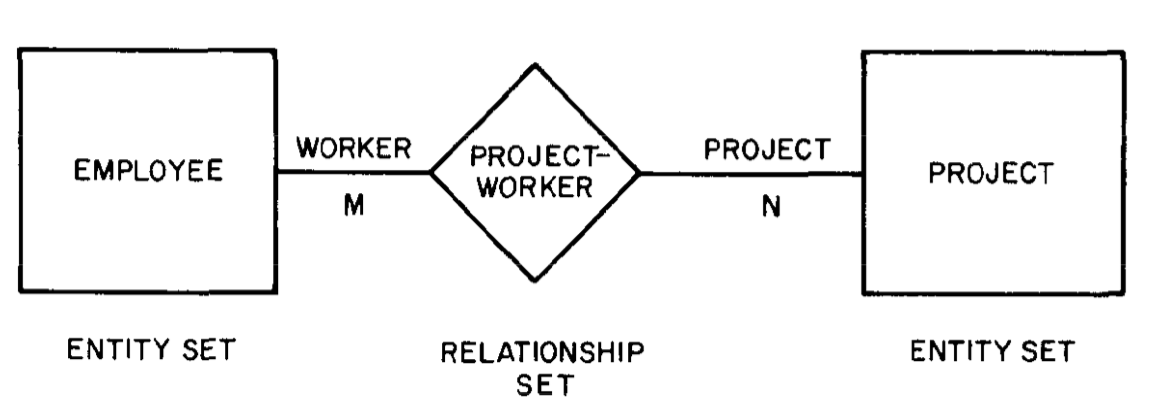
\includegraphics[width=0.6\textwidth]{img/er-bsp.png}
  \end{center}
\end{frame}


%------------------------------------------------------------------------------
\begin{frame}{ER example for a book}

\footnotesize
\begin{tikzpicture}[node distance=6.5em]
%--------------------
% the book
%--------------------
\node[entity](book){Book};
\node[attribute](isbn)[left of=book]{\key{ISBN}} edge(book);
\node[attribute](title)[above left of=book]{title} edge(book);
\node[attribute](pagenr)[above of=book]{nr. of pages} edge(book);

%--------------------
% published by publisher
%--------------------
\node[relationship](published)[below of=book, yshift =-2em]{published} edge node[above right]{N}(book);
\node[entity](publisher)[below of=published, yshift =-2em]{publisher} edge node[above right]{1}(published);
\node[attribute](tid)[left of=publisher]{\key{ID}} edge(publisher);
\node[attribute](tname)[right of=publisher]{Name} edge(publisher);
\node[attribute](address)[above right of=publisher]{address} edge(publisher);
\node[attribute](street)[above right of=address]{Street} edge(address);
\node[attribute](city)[right of=address]{City} edge(address);
\node[multi attribute](phonenr)[below right of=publisher]{phone number} edge(publisher);

%--------------------
% written by author
%--------------------
\node[relationship](written)[right of=  book, xshift =3em]{written} edge node[above right]{N}(book);
\node[entity](author)[right of= written, xshift =3em]{author} edge node[above right]{M}(written);
\node[attribute](birthday)[above  of=author]{birthday} edge(author);
\node[attribute](name)[above right of=author]{name} edge(author);
\node[derived attribute](age)[right of=author]{Age} edge(author);
\end{tikzpicture}

\framebreak 

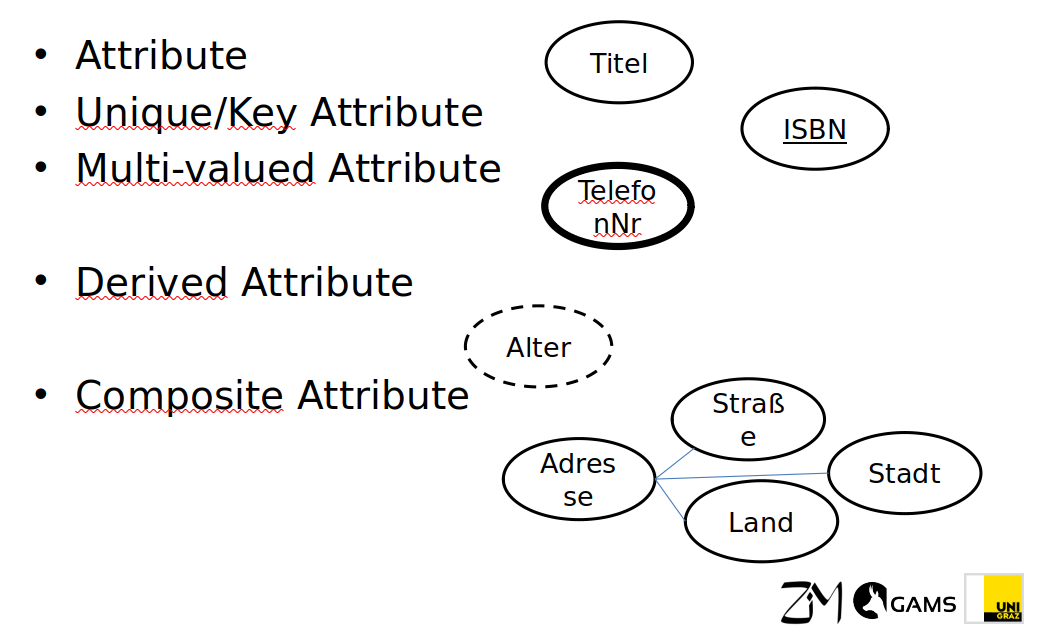
\includegraphics[width=\textwidth]{img/wdh-er-bestandteile.png}

\end{frame}

%------------------------------------------------------------------------------
\begin{frame}{ER example for a book}
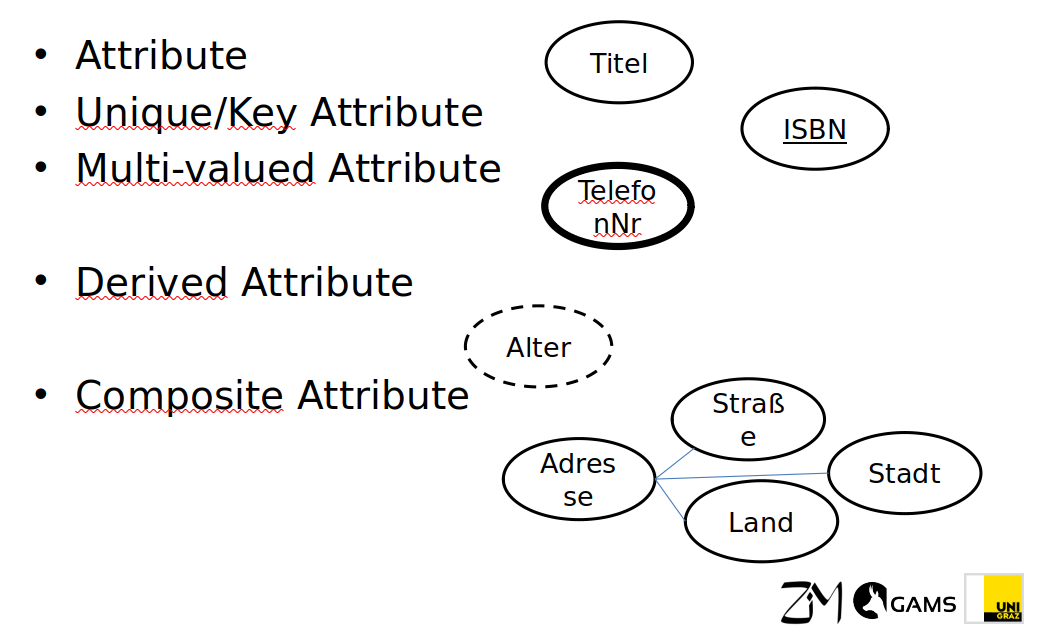
\includegraphics[width=\textwidth]{img/wdh-er-bestandteile.png}

\end{frame}



%------------------------------------------------------------------------------
\begin{frame}[fragile]{Examples}
\metroset{block=fill}
\begin{block}{Entities: university class}
    \begin{itemize}
        \item \textbf{entities:} class, teacher, students, room 
        \item \textbf{attributes:} class (nr., title), teacher (name), students (name, student nr, degree programme, module), room (nr, building, seats) 
        \item \textbf{relations:}
        \begin{itemize}
            \item Teacher teaches class. Ein Kurs wird abgehalten von Dozent:in.
            \item Class happens in room.
            \item Students participate in class. 
        \end{itemize}
    \end{itemize}
\end{block}

\begin{block}{csv example: birth place}\scriptsize
    \begin{verbatim}
    "Name","Address","Description","Longitude","Latitude"
    "forname surname","example street 1, postcode","birth place","7.018242","50.678667"
    \end{verbatim}
    \end{block}
\end{frame}
%------------------------------------------------------------------------------
\begin{frame}{Homework: CSV}
\metroset{block=fill}
    \begin{alertblock}{Assignment}
    \begin{enumerate}\footnotesize
        \item Represent attributes (properties and relations) of your original in a computer processable table (\texttt{.csv} file).
        %Repräsentieren Sie die Attribute (Eigenschaften und Relationen) Ihres Originals mithilfe einer vom Computer zu verarbeitenden Tabelle (CSV-Datei).
        \item To do that, put your attributes in a simple text-only file in a simple text editor (don't do this in MS Word or the like!), saving the file as \texttt{.txt} or \texttt{.csv} (UTF-8 encoding) or export from a table/sheet software like GoogleSheets, LIbre/OpenOffice Calc or Excel. 
    \end{enumerate}
\end{alertblock}

\begin{block}{Please note:}\tiny
Keep in mind that you can only represent attributes in a limited way using CSV:

You can representt the type of relatinship (e.g. `made of', `instance-class-relationship', `bigger-than', etc.) using suitable labels in the CSV header and true/false answers as values for the cells -- but you can't (at this point) say which relationships link entities (such as molecule -- made of -- H).

Relational databases allow for this more complete form of representation between entities using their relationships. For this homework, picking something that will easily fit in to this list / Excel sheet type format will suffice. 
\end{block}
\end{frame}


%------------------------------------------------------------------------------
\begin{frame}[standout]
    \alert{Action!} \\
    Let's install SQLite3 and try out the terminal.
\end{frame}
